% Le chapitre introduction de ma thèse
\chapter{La Limace de mer}
\epigraph{S'il n'y a pas solution, c'est qu'il n'y a pas de problème}{Les Shadoks}

\section{Une partie}
\lipsum[1-2]

\section{La limace de mer}
\begin{figure}[h]
\begin{center}
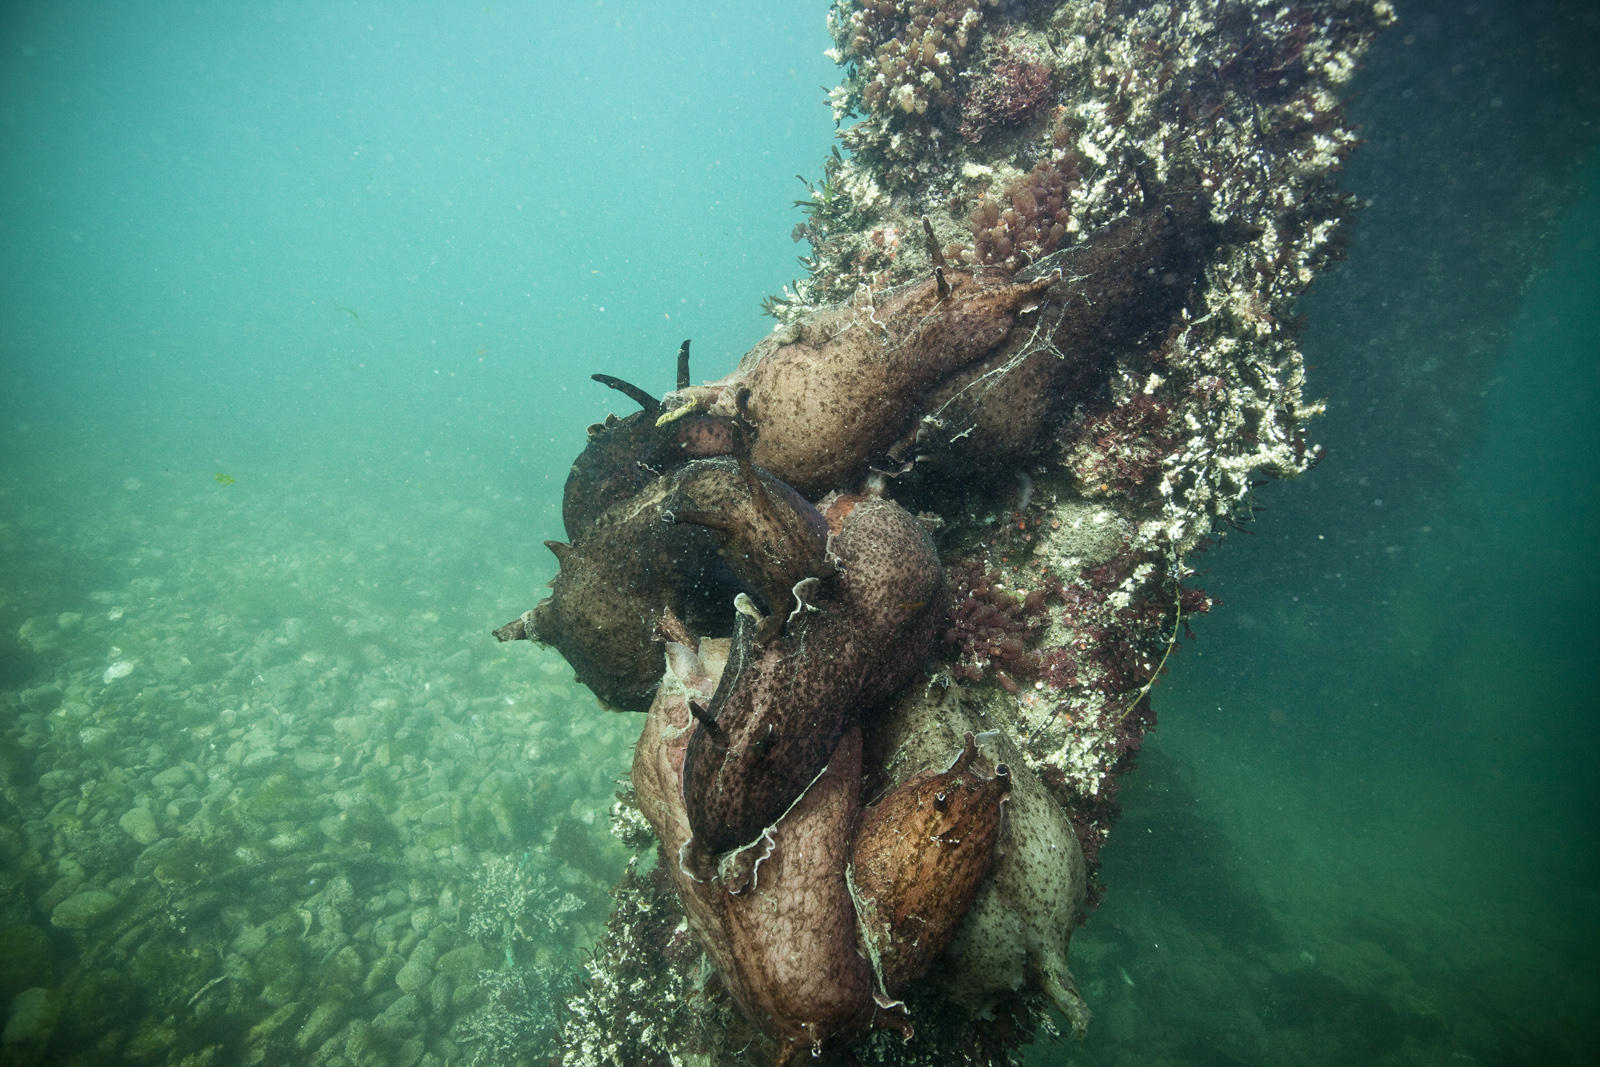
\includegraphics[width = .5\textwidth]{Chap1/figures/limace}
\end{center}
\caption{Un animal marin très intéressant}
\label{fig:limace}
\end{figure}

On observe la figure \ref{fig:limace} (page \pageref{fig:limace}) qui est très explicite\footnote{\href{https://fr.wikipedia.org/wiki/Aplysia}{Wikipedia}}. Un très bon article de Johnson \cite{Johnson, Zoran}, \citep[chapitre 3]{Johnson}.
\lipsum[1-2]

\section{L'autre limace de mer}
\lipsum[2-4]

\section{L'autre limace de mer}
\lipsum[2-5]